%%%%%%%%%%%%%%%%%%%%%%%%%%%%%%%%%%%%%%%%%%%%%%%%%%%%%%%%%%%%%%%%%%%%%%
%
% Title
% PhD Dissertation
% Author
%
% Compile with
% latex/pdflatex thesis
% bibtex thesis
% latex/pdflatex thesis
% latex/pdflatex thesis
%
% Use ``latex'' if you use postscript images
% Use ``pdflatex'' otherwise
%
%%%%%%%%%%%%%%%%%%%%%%%%%%%%%%%%%%%%%%%%%%%%%%%%%%%%%%%%%%%%%%%%%%%%%%

% The default parameters are: 12pt,oneside,doublespace
\documentclass[12pt,twoside,doublespace]{uvathesis}

% The following allows for typical AAS-journal citation methods.
\usepackage{natbib}
\bibliographystyle{aasjournal}

% Some other useful packages
\usepackage{amsmath}
\usepackage{amssymb}
\usepackage{afterpage}
\usepackage{emptypage}

% Load user-defined macros (e.g., journal abbreviations)
\input macros.tex

% Suppress warnings about PDF page groups
\pdfsuppresswarningpagegroup=1

% Footer images with filename ``footer/image_X''
% where X is like 1.jpg, ..., 10.jpg, ..., 100.jpg
% \footerimage{footer/image_}

% Title page information
\title{My Title Here \\ {\normalsize Draft: \today}}
\author{My Full Name}
\hometown{My Hometown, My Home State}
\bachelors{B.A. Astronomy, Cool School, 20XX}
\masters{M.S. Astronomy, University of Virginia, 20X}
\masterstwo{} % If you have a second masters degree
\department{Department of Astronomy}
\degreename{Doctor of Philosophy}
\commencementmonthyear{May 20XX} % This is the month of final exercises
\commencementdate{May XX, 20XX} % This is the date of final exercises

% Committee Members. First one should be PhD advisor
\committeeone{My Advisor}
\committeetwo{Member No. 1}
\committeethree{Member No. 2}
\committeefour{Member No. 3}
\committeefive{Member No. 4}

%%%%%%%%%%%%%%%%%%%%%%%%%%%%%%%%%%%%%%%%%%%%%%%%%%%%%%%%%%%%%%%%%%%%%%
%
% Beginning of document
%
%%%%%%%%%%%%%%%%%%%%%%%%%%%%%%%%%%%%%%%%%%%%%%%%%%%%%%%%%%%%%%%%%%%%%%
\begin{document}

% Make title and copyright page
\frontmatter
\maketitle
\makecopyright

% Make abstract page. Parameter should be name of file containing
% the abstract (without file extension)
\makeabstract{abstract}

% Optional: Make acknowledgements page. Parameter should be name of
% file containing the acknowledgements (without file extension)
\makeacknowledgements{acknowledgements}

% Optional: Make dedications page. Parameter should be dedication
% text.
\makededication{Here's my dedication}

% Make Table of Contents, List of Figures, and List of Tables
\cleardoublepage
\tableofcontents
\cleardoublepage
\listoffigures
\cleardoublepage
\listoftables

% Begin body of document
\mainmatter

% Include each chapter located in
% chapter_X/chapter_X.tex
\cleardoublepage
\chapter{Introduction} \label{chap:intro}

\section{First Section}

Blah blah blah \citep{galilei1610}.

\begin{figure}[p]
  \centering
  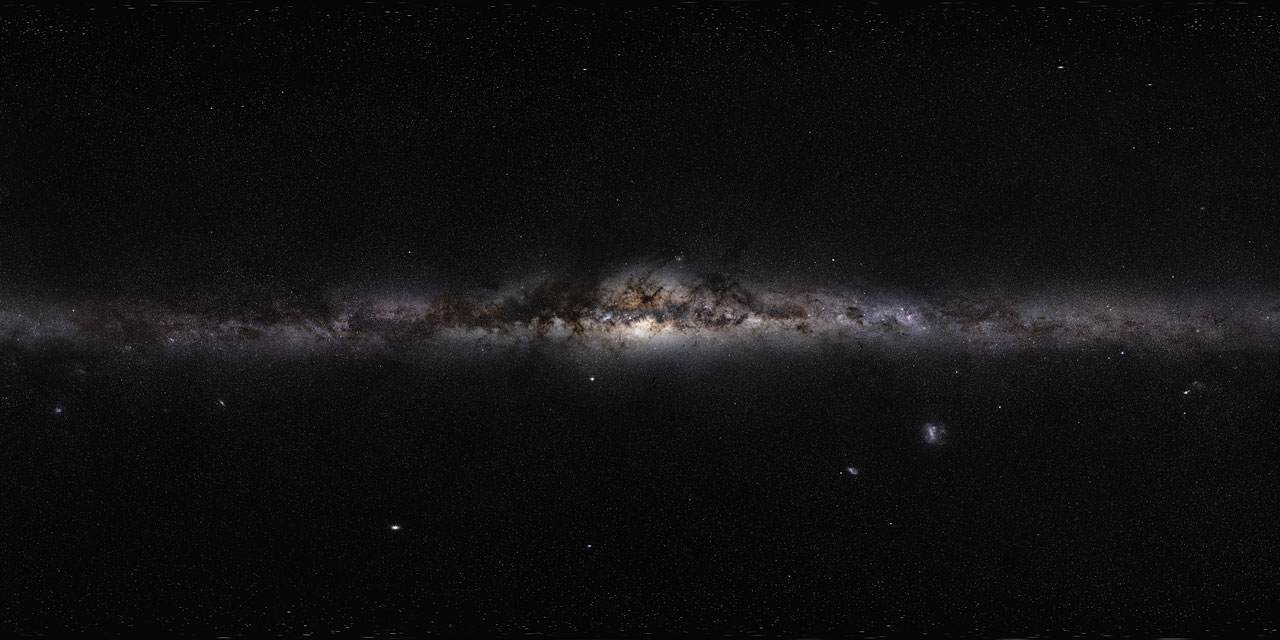
\includegraphics[width=\textwidth]{chapter_1/figures/milkyway.jpg}
  \caption[Short Caption for list of Figures]{Long caption}
  \label{fig:chap1_milkyway}
\end{figure}
\afterpage{\clearpage}

\cleardoublepage
\chapter{Here's Chapter 2!} \label{chap:something_cool}

\section{This is a section}

Blah blah blah

\subsection{This is a subsection}

Blah blah blah


\cleardoublepage
\chapter{Chapter with Tables!} \label{chap:chapter3}

\section{Section with Tables}

Blah blah blah here comes a table.

% Use ``afterpage'' so that the table doesn't interrupt text.
\afterpage{%%%%%%% Here's what you use for a normal, 1-page, portrait table
%
% \begin{thesistable}{lcccr@{\,\(\pm\)\,}lr@{\,\(\pm\)\,}lr}
%
%%%%%%% multi-page portrait
%
% \begin{longthesistable}{lcccr@{\,\(\pm\)\,}lr@{\,\(\pm\)\,}lr}
%
%%%%%%% 1-page landscape
%
% \begin{thesistable}{lcccr@{\,\(\pm\)\,}lr@{\,\(\pm\)\,}lr}
% \rotatetable
%
% And this table is multi-page landscape
\begin{longthesistable}{lcccr@{\,\(\pm\)\,}lr@{\,\(\pm\)\,}lr}
\rotatetable
\tablespacing{\singlespacing}
\tabletypesize{\normalsize}
\tablecaption[High-mass Star Forming Region Sample]{HMSFR Sample}
\tablelabel{\label{tab:chap2_sample}}
\tablehead{
\colhead{Name} & \colhead{Alias} & \colhead{RA (J2000)} & \colhead{Decl. (J2000)} & \multicolumn{2}{c}{Parallax} & \multicolumn{2}{c}{V} & \colhead{Refs.} \\
\colhead{} & \colhead{} & \colhead{(hh:mm:ss)} & \colhead{(dd:mm:ss)} & \multicolumn{2}{c}{(mas)} & \multicolumn{2}{c}{(km s\(^{-1}\))} & \colhead{}
}
\tabledata{
G015.03\(-\)00.67 & M 17            & 18:20:24.81 & \(-\)16:11:35.3 & 0.505 & 0.033 & 22 & 3 & 10 \\
G016.58\(-\)00.05 &  & 18:21:09.08 & \(-\)14:31:48.8 & 0.279 & 0.023 & 60 & 5 & 4 \\
G023.00\(-\)00.41 &  & 18:34:40.20 & \(-\)09:00:37.0 & 0.218 & 0.017 & 80 & 3 & 11 \\
G023.44\(-\)00.18 &  & 18:34:39.19 & \(-\)08:31:25.4 & 0.170 & 0.032 & 97 & 3 & 11 \\
G023.65\(-\)00.12 &  & 18:34:51.59 & \(-\)08:18:21.4 & 0.313 & 0.039 & 83 & 3 & 12 \\
G023.70\(-\)00.19 &  & 18:35:12.36 & \(-\)08:17:39.5 & 0.161 & 0.024 & 73 & 5 & 7 \\
G025.70+00.04 &  & 18:38:03.14 & \(-\)06:24:15.5 & 0.098 & 0.029 & 93 & 5 & 4 \\
G027.36\(-\)00.16 &  & 18:41:51.06 & \(-\)05:01:43.4 & 0.125 & 0.042 & 92 & 3 & 10 \\
G028.86+00.06 &  & 18:43:46.22 & \(-\)03:35:29.6 & 0.135 & 0.018 & 100 & 10 & 4 \\
G029.86\(-\)00.04 &  & 18:45:59.57 & \(-\)02:45:06.7 & 0.161 & 0.020 & 100 & 3 & 6 \\
G029.95\(-\)00.01 & W 43S           & 18:46:03.74 & \(-\)02:39:22.3 & 0.190 & 0.019 & 98 & 3 & 6 \\
G031.28+00.06 &  & 18:48:12.39 & \(-\)01:26:30.7 & 0.234 & 0.039 & 109 & 3 & 6 \\
G031.58+00.07 & W 43Main        & 18:48:41.68 & \(-\)01:09:59.0 & 0.204 & 0.030 & 96 & 5 & 6 \\
G032.04+00.05 &  & 18:49:36.58 & \(-\)00:45:46.9 & 0.193 & 0.008 & 97 & 5 & 4 \\
G033.64\(-\)00.22 &  & 18:53:32.56 & +00:31:39.1 & 0.153 & 0.017 & 60 & 3 & 1 \\
G034.39+00.22 &  & 18:53:18.77 & +01:24:08.8 & 0.643 & 0.049 & 57 & 5 & 13 \\
G035.02+00.34 &  & 18:54:00.67 & +02:01:19.2 & 0.430 & 0.040 & 52 & 5 & 2 \\
G035.19\(-\)00.74 &  & 18:58:13.05 & +01:40:35.7 & 0.456 & 0.045 & 30 & 7 & 14 \\
G035.20\(-\)01.73 &  & 19:01:45.54 & +01:13:32.5 & 0.306 & 0.045 & 42 & 3 & 14 \\
G037.43+01.51 &  & 18:54:14.35 & +04:41:41.7 & 0.532 & 0.021 & 41 & 3 & 2 \\
G043.16+00.01 & W 49N           & 19:10:13.41 & +09:06:12.8 & 0.090 & 0.007 & 10 & 5 & 15 \\
G043.79\(-\)00.12 & OH 43.8\(-\)0.1     & 19:11:53.99 & +09:35:50.3 & 0.166 & 0.005 & 44 & 10 & 2 \\
G043.89\(-\)00.78 &  & 19:14:26.39 & +09:22:36.5 & 0.121 & 0.020 & 54 & 5 & 2 \\
G045.07+00.13 &  & 19:13:22.04 & +10:50:53.3 & 0.125 & 0.005 & 59 & 5 & 2 \\
G045.45+00.05 &  & 19:14:21.27 & +11:09:15.9 & 0.119 & 0.017 & 55 & 7 & 2 \\
G048.60+00.02 &  & 19:20:31.18 & +13:55:25.2 & 0.093 & 0.005 & 18 & 5 & 15 \\
G049.19\(-\)00.33 &  & 19:22:57.77 & +14:16:10.0 & 0.189 & 0.007 & 67 & 5 & 2 \\
G049.48\(-\)00.36 & W 51 IRS2       & 19:23:39.82 & +14:31:05.0 & 0.195 & 0.071 & 56 & 3 & 16 \\
G049.48\(-\)00.38 & W 51M           & 19:23:43.87 & +14:30:29.5 & 0.185 & 0.010 & 58 & 4 & 17 \\
G052.10+01.04 & IRAS 19213+1723 & 19:23:37.32 & +17:29:10.5 & 0.251 & 0.060 & 42 & 5 & 18 \\
G059.78+00.06 &  & 19:43:11.25 & +23:44:03.3 & 0.463 & 0.020 & 25 & 3 & 16 \\
G069.54\(-\)00.97 & ON 1            & 20:10:09.07 & +31:31:36.0 & 0.406 & 0.013 & 12 & 5 & 19,20,21 \\
G074.03\(-\)01.71 &  & 20:25:07.11 & +34:49:57.6 & 0.629 & 0.017 & 5 & 5 & 21 \\
G075.29+01.32 &  & 20:16:16.01 & +37:35:45.8 & 0.108 & 0.005 & -58 & 5 & 22 \\
G075.76+00.33 &  & 20:21:41.09 & +37:25:29.3 & 0.285 & 0.022 & -9 & 9 & 21 \\
G075.78+00.34 & ON 2N           & 20:21:44.01 & +37:26:37.5 & 0.261 & 0.030 & 1 & 5 & 23 \\
G076.38\(-\)00.61 &  & 20:27:25.48 & +37:22:48.5 & 0.770 & 0.053 & -2 & 5 & 21 \\
G078.12+03.63 & IRAS 20126+4104 & 20:14:26.07 & +41:13:32.7 & 0.610 & 0.030 & -4 & 5 & 24 \\
G078.88+00.70 & AFGL 2591       & 20:29:24.82 & +40:11:19.6 & 0.300 & 0.024 & -6 & 7 & 25 \\
G079.73+00.99 & IRAS 20290+4052 & 20:30:50.67 & +41:02:27.5 & 0.737 & 0.062 & -3 & 5 & 25 \\
G079.87+01.17 &  & 20:30:29.14 & +41:15:53.6 & 0.620 & 0.027 & -5 & 10 & 21 \\
G080.79\(-\)01.92\tablenotemark{a} & NML Cyg         & 20:46:25.54 & +40:06:59.4 & 0.620 & 0.047 & -3 & 3 & 26 \\
G080.86+00.38 & DR 20           & 20:37:00.96 & +41:34:55.7 & 0.687 & 0.038 & -3 & 5 & 25 \\
G081.75+00.59 & DR 21           & 20:39:01.99 & +42:24:59.3 & 0.666 & 0.035 & -3 & 3 & 25 \\
G081.87+00.78 & W 75N           & 20:38:36.43 & +42:37:34.8 & 0.772 & 0.042 & 7 & 3 & 25 \\
G090.21+02.32 &  & 21:02:22.70 & +50:03:08.3 & 1.483 & 0.038 & -3 & 5 & 21 \\
G092.67+03.07 &  & 21:09:21.73 & +52:22:37.1 & 0.613 & 0.020 & -5 & 10 & 21 \\
G094.60\(-\)01.79 & AFGL 2789       & 21:39:58.27 & +50:14:21.0 & 0.280 & 0.030 & -46 & 5 & 18,28 \\
G095.29\(-\)00.93 &  & 21:39:40.51 & +51:20:32.8 & 0.205 & 0.015 & -38 & 5 & 28 \\
G097.53+03.18 &  & 21:32:12.43 & +55:53:49.7 & 0.133 & 0.017 & -73 & 5 & 27 \\
G100.37\(-\)03.57 &  & 22:16:10.37 & +52:21:34.1 & 0.291 & 0.010 & -37 & 10 & 28 \\
G105.41+09.87 &  & 21:43:06.48 & +66:06:55.3 & 1.129 & 0.063 & -10 & 5 & 21 \\
G107.29+05.63 & IRAS 22198+6336 & 22:21:26.73 & +63:51:37.9 & 1.288 & 0.107 & -11 & 5 & 29 \\
G108.18+05.51 & L 1206          & 22:28:51.41 & +64:13:41.3 & 1.289 & 0.153 & -11 & 3 & 19 \\
G108.20+00.58 &  & 22:49:31.48 & +59:55:42.0 & 0.229 & 0.028 & -49 & 5 & 28 \\
G108.47\(-\)02.81 &  & 23:02:32.08 & +56:57:51.4 & 0.309 & 0.010 & -54 & 5 & 28 \\
G108.59+00.49 &  & 22:52:38.30 & +60:00:52.0 & 0.398 & 0.031 & -52 & 5 & 28 \\
G109.87+02.11 & Cep A           & 22:56:18.10 & +62:01:49.5 & 1.430 & 0.080 & -7 & 5 & 30 \\
G111.23\(-\)01.23 &  & 23:17:20.79 & +59:28:47.0 & 0.288 & 0.044 & -53 & 10 & 28 \\
G111.25\(-\)00.76 &  & 23:16:10.36 & +59:55:28.5 & 0.294 & 0.016 & -43 & 5 & 28 \\
G111.54+00.77 & NGC 7538        & 23:13:45.36 & +61:28:10.6 & 0.378 & 0.017 & -57 & 5 & 30 \\
G121.29+00.65 & L 1287          & 00:36:47.35 & +63:29:02.2 & 1.077 & 0.039 & -23 & 5 & 19 \\
G122.01\(-\)07.08 & IRAS 00420+5530 & 00:44:58.40 & +55:46:47.6 & 0.460 & 0.020 & -50 & 5 & 31 \\
G123.06\(-\)06.30 & NGC 281         & 00:52:24.70 & +56:33:50.5 & 0.355 & 0.030 & -30 & 5 & 32 \\
G123.06\(-\)06.30 & NGC 281W        & 00:52:24.20 & +56:33:43.2 & 0.421 & 0.022 & -29 & 3 & 19 \\
G133.94+01.06 & W 3OH           & 02:27:03.82 & +61:52:25.2 & 0.512 & 0.010 & -47 & 3 & 33,34 \\
G134.62\(-\)02.19\tablenotemark{a} & S Per           & 02:22:51.71 & +58:35:11.4 & 0.413 & 0.017 & -39 & 5 & 35 \\
G135.27+02.79 & WB 89\(-\)437       & 02:43:28.57 & +62:57:08.4 & 0.167 & 0.011 & -72 & 3 & 36 \\
G209.00\(-\)19.38 & Orion Nebula    & 05:35:15.80 & \(-\)05:23:14.1 & 2.410 & 0.030 & 3 & 5 & 43,44,45 \\
G211.59+01.05 &  & 06:52:45.32 & +01:40:23.1 & 0.228 & 0.007 & 45 & 5 & 1 \\
G229.57+00.15 &  & 07:23:01.84 & \(-\)14:41:32.8 & 0.221 & 0.014 & 47 & 10 & 28 \\
G232.62+00.99 &  & 07:32:09.78 & \(-\)16:58:12.8 & 0.596 & 0.035 & 21 & 3 & 40 \\
G236.81+01.98 &  & 07:44:28.24 & \(-\)20:08:30.2 & 0.298 & 0.018 & 43 & 7 & 28 \\
G239.35\(-\)05.06\tablenotemark{a} & VY CMa          & 07:22:58.33 & \(-\)25:46:03.1 & 0.855 & 0.057 & 20 & 3 & 46,47 \\
G240.31+00.07 &  & 07:44:51.92 & \(-\)24:07:41.5 & 0.212 & 0.021 & 67 & 5 & 28 \\
}
\tablenotetext{a}{Red supergiants}
\tablerefs{
  (1) BeSSeL Survey unpublished; (2) \citet{wu2014};
  (4) \citet{sato2014}; (6) \citet{zhang2014}; (7) \citet{sanna2014};
  (10) \citet{xu2011}; (11) \citet{brunthaler2009}; (12)
  (12) \citet{bartkiewicz2008}; (13) \citet{kurayama2011};
  (14) \citet{zhang2009}; (15) \citet{zhang2013};
  (16) \citet{xu2009}; (17) \citet{sato2010}; (18) \citet{oh2010};
  (19) \citet{rygl2010}; (20) \citet{nagayama2011};
  (21) \citet{xu2013}; (22) \citet{sanna2012}; (23) \citet{ando2011};
  (24) \citet{moscadelli2011}; (25) \citet{rygl2012};
  (26) \citet{zhang2012b}; (27) \citet{hachisuka2015};
  (28) \citet{choi2014}; (29) \citet{hirota2008};
  (30) \citet{moscadelli2009}; (31) \citet{moellenbrock2009};
  (32) \citet{sato2008}; (33) \citet{xu2006};
  (34) \citet{hachisuka2006}; (35) \citet{asaki2010};
  (36) \citet{hachisuka2009}; (40) \citet{reid2009a};
  (43) \citet{sandstrom2007}; (44) \citet{menten2007};
  (45) \citet{kim2008}; (46) \citet{choi2008};
  (47) \citet{zhang2012a}
}
\end{longthesistable}
\clearpage
}




% Begin the appendix
\begin{appendices}
  % Include the appendix located in
  % appendix_X/appendix_X.tex
  \cleardoublepage
  \chapter{Here's my Appendix! \label{sec:appendixA}}

Blah blah blah appendix.

\begin{figure}[p]
  \centering
  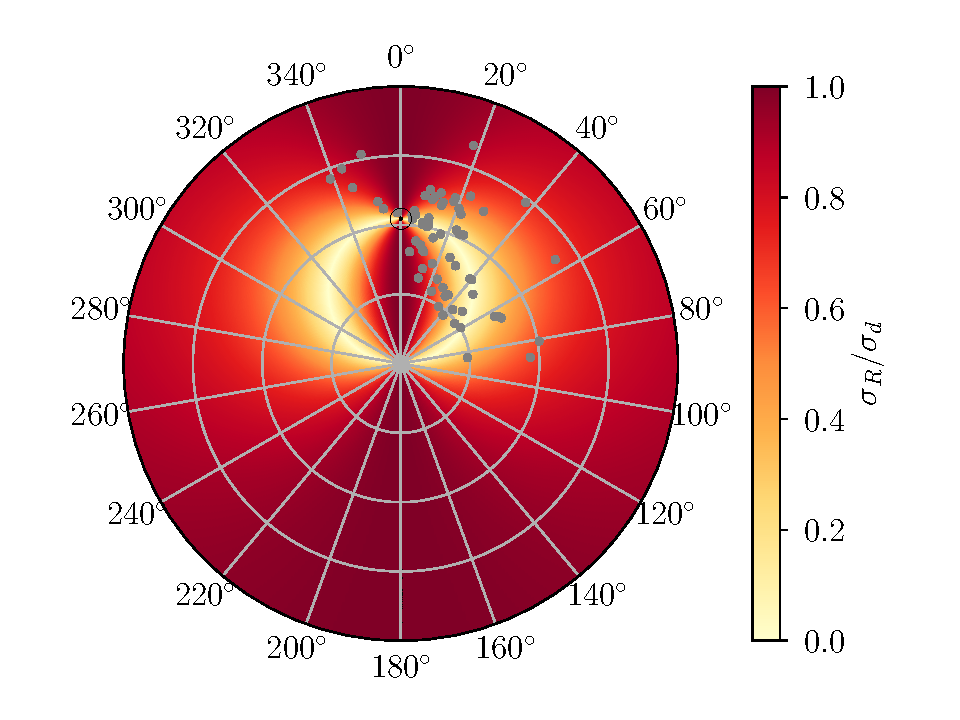
\includegraphics[width=0.75\linewidth]{appendix_A/figures/faceon_rgal.pdf}
  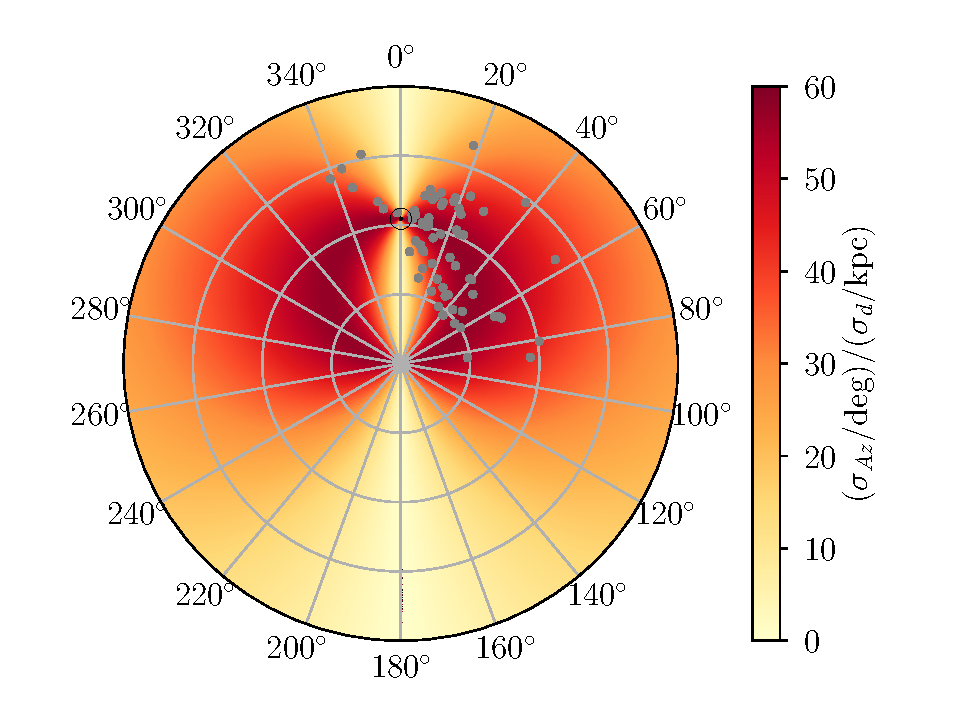
\includegraphics[width=0.75\linewidth]{appendix_A/figures/faceon_az.pdf}
  \caption[Short Caption]{Long caption}
  \label{fig:appA_faceon_unc}
\end{figure}
\afterpage{\clearpage}

\end{appendices}

%
% Load the bibliography, biographical sketch, and CV
%
\makereferences{thesis}
\makebiosketch{biosketch}
\makecv{cv}

\end{document}
